\documentclass[9pt]{beamer}
% Created By Gouthaman KG
%~~~~~~~~~~~~~~~~~~~~~~~~~~~~~~~~~~~~~~~~~~~~~~~~~~~~~~~~~~~~~~~~~~~~~~~~~~~~~~
% Use roboto Font (recommended)
\usepackage[sfdefault]{roboto}
\usepackage[utf8]{inputenc}
\usepackage[T1]{fontenc}
%~~~~~~~~~~~~~~~~~~~~~~~~~~~~~~~~~~~~~~~~~~~~~~~~~~~~~~~~~~~~~~~~~~~~~~~~~~~~~~

%~~~~~~~~~~~~~~~~~~~~~~~~~~~~~~~~~~~~~~~~~~~~~~~~~~~~~~~~~~~~~~~~~~~~~~~~~~~~~~
% Define where theme files are located. ('/styles')
\usepackage{styles/fluxmacros}
\usefolder{styles}
% Use Flux theme v0.1 beta
% Available style: asphalt, blue, red, green, gray 
\usetheme[style=asphalt]{flux}
%~~~~~~~~~~~~~~~~~~~~~~~~~~~~~~~~~~~~~~~~~~~~~~~~~~~~~~~~~~~~~~~~~~~~~~~~~~~~~~

%~~~~~~~~~~~~~~~~~~~~~~~~~~~~~~~~~~~~~~~~~~~~~~~~~~~~~~~~~~~~~~~~~~~~~~~~~~~~~~
% Extra packages for the demo:
\usepackage{booktabs}
\usepackage{colortbl}
\usepackage{ragged2e}
\usepackage{schemabloc}
\usepackage{hyperref}
\usebackgroundtemplate{
\includegraphics[width=\paperwidth,height=\paperheight]{assets/background.jpg}}%change this to your preferred background for the presentation.
%~~~~~~~~~~~~~~~~~~~~~~~~~~~~~~~~~~~~~~~~~~~~~~~~~~~~~~~~~~~~~~~~~~~~~~~~~~~~~~

%~~~~~~~~~~~~~~~~~~~~~~~~~~~~~~~~~~~~~~~~~~~~~~~~~~~~~~~~~~~~~~~~~~~~~~~~~~~~~~
% Informations
\title{CORD-19 DATASET}
\subtitle{AN APPLICATION OF CLUSTERING METHODS}

\author{Quynh Anh Nguyen }
\institute{University of Milan}
\titlegraphic{assets/unimi.eps} %change this to your preferred logo or image(the image is located on the top right corner).

%~~~~~~~~~~~~~~~~~~~~~~~~~~~~~~~~~~~~~~~~~~~~~~~~~~~~~~~~~~~~~~~~~~~~~~~~~~~~~~

\begin{document}

% Generate title page
\titlepage

\begin{frame}

 \frametitle{TABLE OF CONTENTS}
 \tableofcontents
\end{frame}

\section{INTRODUCTION} %the content in the section will be displayed in the table of contents
\begin{frame}{INTRODUCTION}%the content in the frame will be displayed as the title of the page
\begin{itemize}

  \setlength\itemsep{2em}  %increase the space between items.
  
    \item{Dataset} The data set is CORD-19, resource of over 300,000 scholarly articles about COVID19. A subset of 1000 articles will be used in this project.
    
     \item{Goal} Comparing the results of two methods, K-Means and GMM method on clustering 1000 articles and extracting the topic of each cluster.
    
\end{itemize}
    
\end{frame}
\section{METHOD} %the content in the section will be displayed in the table of contents
\begin{frame}{METHOD}%the content in the frame will be displayed as the title of the page
\begin{itemize}

  \setlength\itemsep{1.5em}  %increase the space between items.
  \item Data processing from text into $966\times4096$ matrix.
    \item{PCA }
The number of predictors in the data is much larger than the number of data-points. We apply PCA to reduce the dimension of the data.
    
   \item Finding the best K by Elbow method and Gap Statistics
   
   \item Applying K-Means and GMM for the 2-dimensional projected data.
   
   \item Finding the optimal number of clusters for GMM method by AIC and BIC indicator.
   
   \item Evaluating the performance of both methods by extracting keywords of each cluster and check whether they are describing for a topic. 
    
\end{itemize}
\end{frame}
%%%%%%%%%%%%%%%%%%%%
\section{RESULTS}
\begin{frame}{Tuning the optimal number of cluster}

\subsection{Tuning K}
\begin{figure}
  \centering
  \begin{minipage}[b]{0.4\textwidth}
    \includegraphics[width=1\columnwidth]{2.eps}
    \caption{ Elbow method.}
  \end{minipage}
  \hfill
  \begin{minipage}[b]{0.4\textwidth}
    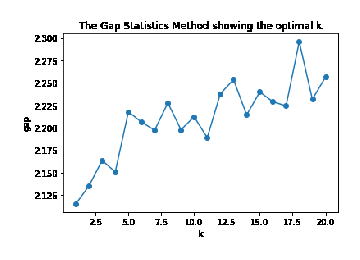
\includegraphics[width=1\columnwidth]{3Gap.eps}
    \caption{ Gap Statistics method.\label{2}}
  \end{minipage}
\end{figure}

    \item Dataset: $966\times708$ matrix 
    \item Distortion: The sum of squared distances from each point to its centroid is computed and plotted against k.
    \item{Gap Statistics: \begin{equation}
Gap(K) = \log W(K) - \log W_{uniform}(K)
\end{equation}}
    
\end{frame}
%%%%%%%%%
\begin{frame}{Keywords of 17 clusters by K-Means}

\begin{figure}
  \begin{minipage}[b]{1.1\textwidth}
    \includegraphics[width=0.8\columnwidth]{4.17cluster.eps}
    \caption{ Keywords of clusters by K-Means \label{4}}
  \end{minipage}
\end{figure}
\end{frame}
%%%%%%%%%
\subsection{K-Means Evaluating}
\begin{frame}{WordCloud of clusters by K-Means}

\begin{figure}
  \begin{minipage}[b]{0.8\textwidth}
    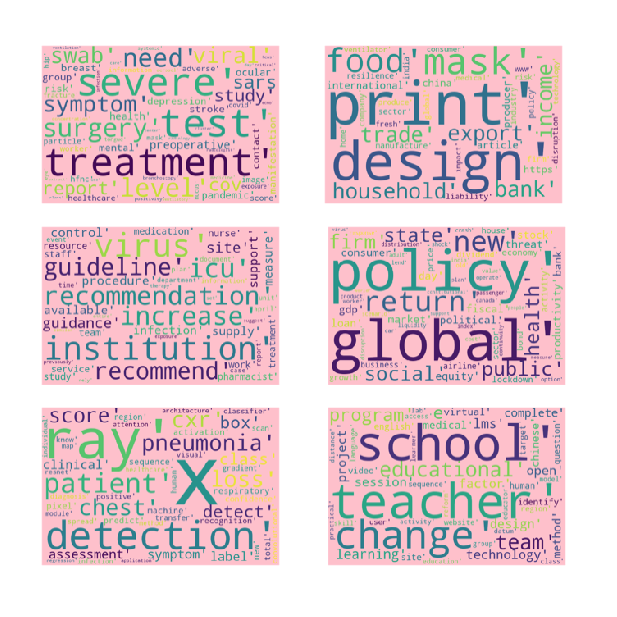
\includegraphics[width=0.8\columnwidth]{5_cloud.eps}
    \caption{ Word-Cloud from Keywords of Clusters by K-Means Method \label{2}}
  \end{minipage}
\end{figure}
la
\end{frame}

\subsection{GMM - K-Means}
\begin{frame}{Plot cluster by K-Means and GMM method}
\begin{figure}[!t]
  \centering
  \begin{minipage}[b]{0.45\textwidth}
    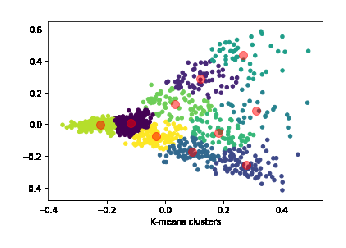
\includegraphics[width=1\columnwidth]{6_kmeans_2dim.eps}
    \caption{ K-Means Method.}
  \end{minipage}
  \hfill
  \begin{minipage}[b]{0.45\textwidth}
    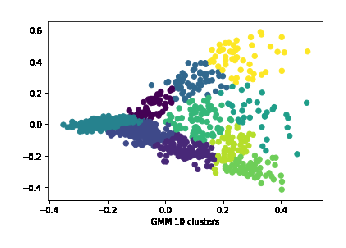
\includegraphics[width=1\columnwidth]{7_gmm_2dim.eps}
    \caption{Gaussian Mixture Method.\label{gmm}}
  \end{minipage}
\end{figure}

    \item Dataset: $966\times2$ matrix 
    \item K-Means method lacks of flexibility in cluster shape and lack of probabilistic cluster assignment. This weakness is improved in GMM method.
\end{frame}

\subsection{BIC &  AIC}
\begin{frame}{Finding optimal component with BIC and AIC indicators}
\begin{figure}[!b]
  \centering
  \begin{minipage}[b]{0.45\textwidth}
    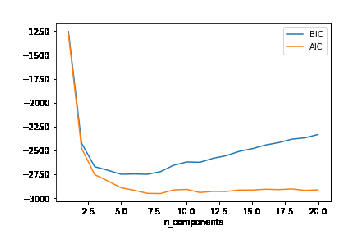
\includegraphics[width=1\columnwidth]{9_gmm_bic.eps}
    \caption{AIC and BIC index.}
  \end{minipage}
  \hfill
  \begin{minipage}[b]{0.45\textwidth}
    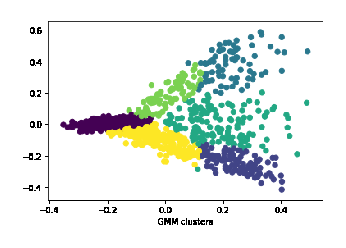
\includegraphics[width=1\columnwidth]{9_mm_scatterplot.eps}
    \caption{n\_component is 6.\label{nqa}}
  \end{minipage}
\end{figure}
     \item Dataset: $966\times2$ matrix 
     \item The optimal numberof clusters is the value that minimizes the AIC or BIC.
\end{frame}
%%%%%%%%%%%%%%%%%%%%%%%%%%%%%%%%%%%%%%%%%%%%%%%%%
\subsection{GMM Evaluating}
\begin{frame}{WordCloud of clusters by GMM method}
\begin{figure}[!t]
  \centering
  \begin{minipage}[b]{1\textwidth}
    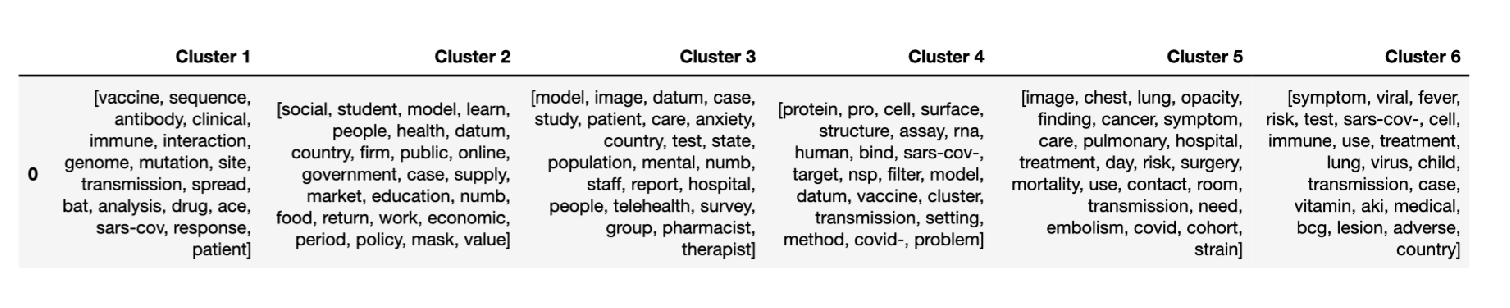
\includegraphics[width=1\columnwidth]{gmm_keywords.eps}
    \caption{Keywords of 6 clusters by GMM method.}
  \end{minipage}
  \hfill
  \begin{minipage}[b]{0.7\textwidth}
    \includegraphics[width=0.5\columnwidth]{gmmz0all.eps}
    \caption{WordCloud of 6 clusters by GMM method\label{nqa}}
  \end{minipage}
\end{figure}
    \item Dataset: Corpus
\end{frame}
%%%%%%%%%%%%%%%%%%
\section{CONCLUSION}
\begin{frame}{CONCLUSION}
\begin{itemize}

  \setlength\itemsep{1em}  %increase the space between items.
  
    \item The optimal number of clusters of K-Means method are 10; whereas it is 6 for GMM model.
    
    \item The GMM model shows the better result on two-dimensional data compared to K-Means method.
    
    \item In reality, the extracted keywords proved that K-Means is the better method.
    
    \item The different results of two methods can be explained by the dimension of the dataset, by the method determine the optimal cluster or components as well.
    
\end{itemize}
\end{frame}
%%%%%%%%%%%%%%%%%%%%%%%%%%%%%%%%%%%%%%%%%%%%%%%%%%%%%%%%%%%%%%%%%%%%%%%%%%%%%%%%%%%%%%%%%%%%%%%%%%%%%%%%%%%%
\section{REFERENCES}
\begin{frame}{REFERENCES}

Manzi, G. (2020), Lecture 20: Course Recap, lecture notes. \textit{Advanced Multivariate Statistics B7416}, University of Milan, delivered December 2020.

 Boehmke, B. \& Greenwell, B. (2020).  Chapter 22 Model-based Clustering. \textit{Hands-On Machine Learning with R}, \url{https://bradleyboehmke.github.io/HOML/model-clustering.html}.
 
 VanderPlas, J. (2016).  In Depth: Gaussian Mixture Models.  \textit{Python Data Science Handbook}, \url{https://jakevdp.github.io/PythonDataScienceHandbook/05.12-gaussian-mixtures.html}.

 MaksimEkin (2020).  Loading data. \textit{COVID-19 Literature Clustering}, \url{https://www.kaggle.com/maksimeren/covid-19-literature-clustering/notebook}.
 
 Palafox, L. (2019).  A visual introduction to the Gap Statistics. \textit{The Glowing Python}, \url{https://glowingpython.blogspot.com/2019/01/a-visual-introduction-to-gap-statistics.html}.

\end{frame}
    

\end{document}